\documentclass[11pt,a4paper,openany,leqno]{article}

\textwidth=160mm \textheight=260mm \hoffset=-18mm \voffset=-30mm
\setcounter{page}{1}
			\usepackage[magyar]{babel}
			\usepackage[utf8]{inputenc}
			\usepackage[T1]{fontenc}
			\usepackage{indentfirst}
			\usepackage{amsmath,esint}
			\usepackage{amssymb}
%			\usepackage{eufrak}
			\usepackage{psfrag}
			\usepackage{tabularx}
			\usepackage{graphicx}
			\usepackage{wrapfig}	
			\usepackage{hyperref}
			\usepackage{multicol}	
									
			\frenchspacing
			\allowhyphens

\tolerance=2000
\hbadness=2000
\vbadness=10000
\overfullrule=0pt




\begin{document}
\section{Optika}
\subsection{Kovács-Párkányi Fizikai Példatár II. / 223. Feladat}
\indent
Határozzuk meg két lencséből álló lencserendszer nagyítását, ha adott a lencsék fókusztávolsága, a lencsék egymástól való távolsága ($d$), és a tárgy távolsága a lencsétől.
\begin{figure}[h!]
\centering
  \includegraphics[width=120mm,scale=0.5]{kep11.pdf}
  \caption{A két lencse és a kép kialakulása}
  \label{}
\end{figure} 
 \indent



\begin{flushright} {Feladatot kidolgozta: {\it Z2R8XS}} \end{flushright}

\vspace{0.5cm}

\textbf{Megoldás}\\
\indent
A feladat nem adta meg konkrétan, milyen lencsékről van szó, viszont ha a képtávolságot és a fókusztávolságot előjelesen használjuk, úgyanúgy érvényesülni fog minden lencsére a levezetés.\\ \indent
Nézzük, milyen összefüggés áll fenn a képtávolság, tárgytávolság és a fókusztávolság között. Legyen $f$ a fókusztávolság, $t$ a tárgy távolsága a lencsétől, $k$ a kép távolsága a lencsétől, $T$ a tárgy mérete és $K$ a kép mérete.\\
\begin{figure}[h!]
\centering
  \includegraphics[width=90mm, scale=0.5]{kep21.pdf}
  \caption{Domború lencse}
  \label{}
\end{figure}\\ 
\indent
Az $ACB$ és a $CED$ háromszögek hasonlóak. Vegyük a két beforgó arányát.\\
$$ \frac{AB}{DE} = \frac{BC}{CD} $$
$$ \frac{T}{K} = \frac{f}{k-f} $$\indent
Az $AFB$ és a $DBE$ háromszögek hasonlóak. Vegyük a két beforgó arányát.\\
$$ \frac{BD}{FA} = \frac{DE}{AB} $$
$$ \frac{k}{t} = \frac{K}{T} = N$$\indent
Az $N$-t szokás a lencse nagyításának nevezni. Használjuk fel ezt a két összefüggést.\\
$$ \frac{t}{k} = \frac{k-f}{f} $$
$$ t\cdot k - t\cdot f = f\cdot k $$
$$ \frac{1}{f} - \frac{1}{k} = \frac{1}{t} $$
$$ \frac{1}{f} = \frac{1}{k} + \frac{1}{t} $$\indent
Nézzük meg, a lencserendszer nagyítása hogy áll elő az őt alkotó két lencse nagyításából.\\ \indent
Az első lencse $T_1$ tárgyról alkot $K_1$ képet: $K_1 = N_1 \cdot T_1$.\\ \indent
A második lencse $T_1$ tárgyról alkot $K_2$ képet: $K_2 = N_2 \cdot T_2$. \\ \indent
Kulcsfontosságú lépés, hogy az első lencse képe (piros $K_1$) a második lencse tárgya (kék $T_2$), azaz $K_1 = T_2$. Innen:\\
$$ K_2 = N_2 \cdot T_2 = N_2 \cdot K_1 = N_2 \cdot (N_1 \cdot T_1) $$\indent
A lencserendszer $T_1$ tárgyról alkot $K_2$ képet, így a rendszer nagyítása:\\
$$ N = \frac{K_2}{T_1} = N_1 \cdot N_2 $$\indent
A lencserendszer nagyítása egyenlő a lencsék nagyításának szorzatával.\\ \indent
A feladat szerint csak $f_1$, $f_2$, $d$ és $t_1$ adott, fejezzük ki ezekkel a nagyítást.\\
$$ N = N_1 \cdot N_2 $$
$$ N = \frac{K_1}{T_1} \cdot \frac{K_2}{T_2} $$
$$ N = \frac{k_1}{t_1} \cdot \frac{k_2}{t_2} $$\indent
$k_1$ kifejezhető az ismert $t_1$-gyel és $f_1$-gyel.\\ 
$$ \frac{1}{f_1} = \frac{1}{k_1} + \frac{1}{t_1} $$
$$ \frac{1}{k_1} = \frac{1}{f_1} - \frac{1}{t_1} $$
$$ k_1 = \frac{f_1 \cdot t_1}{t_1-f_1} $$
\indent
$t_2$ kifejezhető $k_1$-gyel és $d$-vel.\\
$$ t_2+k_1 = d $$
$$ t_2 = d - \frac{f_1 \cdot t_1}{t_1-f_1}  $$
\indent
$k_2$ kifejezhető $t_2$-vel és $f_2$-vel.\\
$$ \frac{1}{f_2} = \frac{1}{k_2} + \frac{1}{t_2} $$
$$ \frac{1}{k_2} = \frac{1}{f_2} - \frac{1}{t_2} $$
$$ k_2 = \frac{f_2 \cdot t_2}{t_2-f_2} $$
$$ k_2 = \frac{f_2 \cdot (d - \frac{f_1 \cdot t_1}{t_1-f_1} )}{(d - \frac{f_1 \cdot t_1}{t_1-f_1})-f_2} $$\indent
Térjünk vissza $N$-hez.\\
$$ N = \frac{k_1}{t_1} \cdot \frac{k_2}{t_2} $$
$$ N = k_1\cdot \frac{1}{t_1} \cdot k_2 \cdot\frac{1}{t_2} $$
$$ N = \frac{f_1 \cdot t_1}{t_1-f_1}\cdot \frac{1}{t_1} \cdot \frac{f_2 \cdot (d - \frac{f_1 \cdot t_1}{t_1-f_1} )}{(d - \frac{f_1 \cdot t_1}{t_1-f_1} )-f_2} \cdot\frac{1}{d - \frac{f_1 \cdot t_1}{t_1-f_1} } $$
$$ N = \frac{f_1 }{t_1-f_1} \cdot \frac{f_2}{(d - \frac{f_1 \cdot t_1}{t_1-f_1} )-f_2} $$\indent
Az alábbi összefüggést kapjuk a lencserendszer nagyítására:\\
$$ N =  \frac{f_1\cdot f_2}{(t_1-f_1)(d-f_2) - t_1\cdot f_1} $$


\newpage

\subsection{Kovács-Párkányi Fizikai Példatár II. / 267. Feladat}
\indent
Az optikai rács $cm$-enként $5700$ rést tartalmaz. Maximálisan hány rend jelenhet meg ennek a rácsnak a színképében, ha látható fénnyel világítjuk meg?
\begin{figure}[h!]
\centering
  \includegraphics[width=120mm,scale=0.5]{kep31.pdf}
  \caption{Rácsra érkező fénysugarak}
  \label{}
\end{figure} 
 \indent

\begin{flushright} {Feladatot kidolgozta: {\it Z2R8XS}} \end{flushright}
\vspace{0.5cm}
\textbf{Megoldás}\\
\indent
A látható fény hullámhossza a $\lambda \in[3,9\cdot 10^{-7}m;7,5\cdot 10^{-7}m]$ intervallumba esik. Keressük egy látható tartományba eső monokromatikus fényhez a maximális rendet, adott $d=10^{-2}m/5700$ rácsállandó mellett.\\ \indent
Az alábbi összefüggés érvényesül a rácsállandó ($d$), a beesési szög ($\theta$), az intentzitásmaximumok iránya ($\beta_k$), a fény hullámhossza ($\lambda$) és a rend ($k$) között.\\
$$ d\cdot (sin(\theta) + sin(\beta_k)) = \pm k\cdot \lambda $$\indent
Érdemes megvizsgálni a szélső eseteket. Legyen merőleges beesés, azaz $\theta = 0$, így $sin(\theta)=0$. Módosítsuk az egyenletet.\\ \indent
$$ d\cdot sin(\beta_k) = \pm k\cdot \lambda $$\indent
Vizsgáljuk a pozitív eseteket. Szimmetrikus jelenségről van szó, tehát ha $k$-t mindig pozitívnak vesszük, egy pozitív $sin(\beta_k)$-hoz tartozó $k$ ugyanaz, mint egy negatív $sin(\beta_k)$-hoz - ha a $\pm$ eseteit ehhez igazítva kezeljük.\\
$$ d\cdot sin(\beta_k) = k\cdot \lambda $$
$$ k = \frac{d\cdot sin(\beta_k)}{\lambda} $$\indent
Technikailag azt kell megoldani, hogy fix $d$ mellett keressük $k$ maximális pozitív egész megoldását, miközben $\lambda$ nem léphet ki a látható tartományból. Megnézzük melyik a legmagasabb elérhető rend, majd ebből kikövetkeztethető, összesen hány rend, illetve hány csík jelenik meg. Tudjuk, hogy $sin(\beta_k)$ maximuma $1$. Az lesz a legszélsőségesebb irány, melynél $sin(\beta_k)$ közelítőleg $1$, itt jelenik meg a legmasabb rend.\\
$$ k = \frac{d}{\lambda} $$\indent
A hullámhossz a nevezőben van, így minél kisebb hullámhosszt kell választani. Meg kell találni azt a legkisebb hullámhosszt, melynél ez a hányados pozitív egész szám lesz.\\
$$ k = \frac{1m}{57\cdot 10^{4}}\cdot\frac{1}{\lambda} $$\indent
Legyen $x = \lambda\cdot 10^{7} $. Így $x$-nek a $[3,9m;7,5m]$ tartományban kell lennie.\\
$$ k = \frac{10^{-4}m}{57}\cdot\frac{1}{x \cdot 10^{-7}} $$
$$ k = \frac{10^{3}m}{57}\cdot\frac{1}{x} $$
$$ k = \frac{10^{3}m}{57\cdot x} $$\indent
Legyen $y = 57\cdot x $. Így $y$-nak a $[222,3m;427,5m]$ tartományban kell lennie.\\
$$ k = \frac{1000m}{y} $$\indent
A probléma arra redukálódott, hogy az $1000$ számnak azt a legkisebb osztóját keressük, mely eleme a $[222,3m;427,5m]$ intervallumnak. Belátható, hogy $y=250m$.\\ \indent
Helyettesítsünk vissza, nézzük mekkora lesz $\lambda$.\\
$$ \lambda = (\frac{y}{57})\cdot 10^{-7} = 4,385964912 \cdot 10^{-7}m = 438,5964912 \cdot 10^{-9}m $$\indent
Tehát a közelítőleg $438,5964912 nm$ hullámhosszú fénynél jelenik meg a legtöbb rend (ez sötétkéknek felel meg). A legmagasabb előforduló rend $k=4$. Mivel nem történik olyan, hogy átugrunk egy rendet (például nem következhet az első után a negyedik), pozitív $sin(\beta_k)$-kra $4$ csík jelenik meg, negatív $sin(\beta_k)$-kra is $4$, és lesz egy $k=0$ eset is, azaz összesen $9$ irányban kapunk intentzitásmaximot, konstruktív interferenciát.





\end{document}